\begin{tikzpicture}[scale=0.5]
\begin{scope}[xshift=0cm, yshift=0cm]

	\def\xmin{-3}
	\def\xmax{3}
	\def\ymin{0}
	\def\ymax{2}
	\def\period{2.0}
	\def\T1{1}
	\def\A{1}
	
	\edef\pulse{|- ++(2*\T1, \A) |- ++( \period - \T1, -\A)}

	
	\draw (\xmin-1, 0) --(\xmax+1, 0) node[anchor=west] {\small $t$};
	\draw (0, \ymin) --(0, \ymax) node[anchor=south] {\small $x_1(t)$};
	\draw[thick] (-3, 0) -- (-\T1,0) -- (-\T1, 1) -- (\T1,1) -- (\T1,0) -- (3,0);
		
		\node at (-\T1, 0) [anchor=north] {\small $-T_1$};
		\node at (\T1, 0) [anchor=north] {\small $T_1$};
		\node at (0, 1) [anchor=south east] {\small $1$};
\end{scope}		
\pause
\begin{scope}[xshift=6cm, yshift=-2cm]	
    \begin{axis}[
		y=4cm,
		x=1cm,
		 clip=false,
		 xmin=-5.5,xmax=5.5,
		 xlabel= $\omega$,
		 ylabel={$X_1(j\omega)$},
		 ymin=-0.5,ymax=1.2,
		 axis lines=middle,
         	%xtick={-5, -4, ..., 5},
		 %ytick={-1, 1},
		 yticklabels=\empty,
		 xticklabels=\empty,
		 every axis x label/.style={at={(ticklabel* cs:1.05)}, anchor=west,},
		every axis y label/.style={at={(ticklabel* cs:1.05)}, anchor=south,},
     ]
		%\addplot+[red, smooth, mark=none] table [x={n}, y={xn}] {periodic_square_fs_samples_of_envilope_gen.dat};
		\addplot [red, thick, domain=-5:5, samples=200] plot{sin(pi*deg(x))/(pi*x)};
		\node at (axis cs:0, 1) [anchor=east] { $2T_1$ };
		\draw[latex-] (axis cs:pi/3, 0) --(axis cs:0.6,-0.3) node  [anchor=north] { $\pi/T_1$ } ;
		\draw[latex-] (axis cs:-pi/3, 0) --(axis cs:-0.6,-0.3) node  [anchor=north] { $-\pi/T_1$ } ;		
    \end{axis}
\end{scope}		

\pause

\begin{scope}[xshift=-5.5cm, yshift=-9cm]
    \begin{axis}[
		y=4cm,
		x=1cm,
		 clip=false,
		 xmin=-5.5,xmax=5.5,
		 xlabel= $t$,
		 ylabel={$x_2t)$},
		 ymin=-0.5,ymax=1.2,
		 axis lines=middle,
         	%xtick={-5, -4, ..., 5},
		 %ytick={-1, 1},
		 yticklabels=\empty,
		 xticklabels=\empty,
		 every axis x label/.style={at={(ticklabel* cs:1.05)}, anchor=west,},
		every axis y label/.style={at={(ticklabel* cs:1.05)}, anchor=south,},
     ]
		%\addplot+[red, smooth, mark=none] table [x={n}, y={xn}] {periodic_square_fs_samples_of_envilope_gen.dat};
		\addplot [red, thick, domain=-5:5, samples=200] plot{sin(pi*deg(x))/(pi*x)};
		\node at (axis cs:0, 1) [anchor=east] { $W/\pi$ };
		\draw[latex-] (axis cs:pi/3, 0) --(axis cs:0.6,-0.3) node  [anchor=north] { $\pi/W$ } ;
		\draw[latex-] (axis cs:-pi/3, 0) --(axis cs:-0.6,-0.3) node  [anchor=north] { $-\pi/W$ } ;		
    \end{axis}
\end{scope}	
\pause
\begin{scope}[xshift=11.5cm, yshift=-7cm]

	\def\xmin{-3}
	\def\xmax{3}
	\def\ymin{0}
	\def\ymax{2}
	\def\period{2.0}
	\def\T1{1}
	\def\A{1}
	
	\edef\pulse{|- ++(2*\T1, \A) |- ++( \period - \T1, -\A)}

	
	\draw (\xmin-1, 0) --(\xmax+1, 0) node[anchor=west] {\small $\omega$};
	\draw (0, \ymin) --(0, \ymax) node[anchor=south] {\small $X_2(j\omega)$};
	\draw[thick] (-3, 0) -- (-\T1,0) -- (-\T1, 1) -- (\T1,1) -- (\T1,0) -- (3,0);
		
		\node at (-\T1, 0) [anchor=north] {\small $-W$};
		\node at (\T1, 0) [anchor=north] {\small $W$};
		\node at (0, 1) [anchor=south east] {\small $1$};

\end{scope}
\pause

\node at (5,2) {$\overset{\mathcal{F}}{\longleftrightarrow}$};
\node at (5,-5.5) {$\overset{\mathcal{F}}{\longleftrightarrow}$};
\pause
\draw[double, orange, very thick, -latex] (5, -3) -- ++(45:2);
\draw[double, orange, very thick, -latex] (5, -3) -- ++(-45:2);
\draw[double, orange, very thick, -latex] (5, -3) -- ++(135:2);
\draw[double, orange, very thick, -latex] (5, -3) -- ++(-135:2);
\end{tikzpicture}